\documentclass[11pt]{article}

\usepackage[utf8]{inputenc}
\usepackage[T1]{fontenc}
\usepackage[a4paper,margin=1in]{geometry}
\usepackage{graphicx}
\usepackage{booktabs}
\usepackage{longtable}
\usepackage{tabularx}
\usepackage{array}
\usepackage{float}
\usepackage{caption}
\usepackage{hyperref}
\usepackage{enumitem}
\usepackage{xcolor}

\setlength{\emergencystretch}{2em}
\setlist[itemize]{leftmargin=1.5em}
\setlist[enumerate]{leftmargin=1.5em}
\renewcommand{\arraystretch}{1.18}
\setcounter{tocdepth}{2}

\newcolumntype{Y}{>{\raggedright\arraybackslash}X}

\title{Technical Report on the Implemented \texttt{main\_2} Corrosion Pipeline}
\author{Repository-grounded reconstruction from code, data, artifacts, and local documentation}
\date{\today}

\begin{document}

\maketitle

\begin{abstract}
This report reconstructs the \texttt{main\_2} project strictly from the executable repository state, saved artifacts, generated diagnostics, the current raw workbook, and the local thesis and conference PDFs stored under \texttt{Documentation/}. The implemented system is a current-state corrosion regressor: it predicts the continuous surface label \texttt{B\_Peak\_Rust\_Percentage\_[\%]} for a given image, optionally concatenated with experiment metadata, and exposes the selected model through a FastAPI endpoint for ``current corrosion'' prediction. It does not implement direct image-to-RUL learning, survival analysis, hidden structural damage estimation, or sequence forecasting.

The repository also contains important reproducibility drift. The saved artifacts document one successful run on 792 observations, but the current raw Excel workbook now has two header rows, 791 labeled data rows, no directly exposed \texttt{NaCl\%} column, and a different identifier layout than the loader expects. The single corrupted image \texttt{E01-20240508-17W.png} is still present in the image directory and in the saved predictions, but its label row is absent from the current workbook. The report therefore treats the saved outputs as evidence of what was run, while explicitly marking what can no longer be rerun from the present raw files without code or data repair.
\end{abstract}

\tableofcontents
\clearpage

\section{Problem framing}

\subsection{Actual task implemented in \texttt{main\_2}}
The executable training pipeline in \texttt{main\_2/train\_phase2.py} solves a single supervised regression problem: predict the corrosion label \texttt{B\_Peak\_Rust\_Percentage\_[\%]} for each image-timepoint pair. The selected saved artifact is an image-only multilayer perceptron (MLP) fed by a frozen 512-dimensional ResNet-18 embedding. A second model, named ``multimodal'', concatenates the same image embedding with tabular metadata, but this branch was not selected for deployment in the saved run.

This is not a future forecasting pipeline. The model input image and the target belong to the same observation row, and no target shifting, sequence windowing, autoregressive modeling, or future-week prediction logic appears in the code. The generated ``progression'' plots in \texttt{main\_2/visualize.py} are retrospective diagnostics over already observed weeks; they are not forecast trajectories.

\subsection{What is directly supervised and what is not}
The only direct supervised target in \texttt{main\_2/config.py} is:
\begin{itemize}
  \item \texttt{B\_Peak\_Rust\_Percentage\_[\%]}: a continuous corrosion quantity defined in the workbook and treated as the regression target.
\end{itemize}

The following quantities exist in the current workbook but are not used as learning targets in \texttt{main\_2}:
\begin{itemize}
  \item \texttt{A\_Surface\_Total\_Rust\_Percentage[\%]}
  \item \texttt{A\_Total\_Rust\_Category\_(1--4)}
  \item \texttt{B\_Peak\_Rust\_Category\_(1--4)}
  \item \texttt{B\_Location\_of\_Peak\_Rus\_\ in\_length\_[cm]}
  \item \texttt{Last\_Wire\_Area\_Loss\_(Faliure\_Surface)\_\%}
  \item \texttt{Ultimate\_Load\_[kN]}
\end{itemize}

The structural variables are especially sparse: in the current workbook they appear only once per specimen (48 non-null values each over 791 labeled rows), which makes them endpoint-type measurements rather than dense frame-level supervision. No code in \texttt{main\_2} trains against them, regresses them, thresholds them, or converts them into remaining useful life.

\subsection{Why direct image-to-RUL is not supported}
Direct image-to-RUL is unsupported for three repository-grounded reasons:
\begin{enumerate}
  \item No RUL label exists in the executable pipeline. Neither the workbook nor the artifacts contain a dedicated remaining-life column.
  \item No proxy-RUL logic exists in \texttt{main\_2}. There is no threshold-crossing model, no survival/event-time formulation, no degradation fit, and no time-to-failure loss.
  \item The served API endpoint is explicitly \texttt{/predict/current}, and the inference function is named \texttt{predict\_current\_corrosion}; it clips a current corrosion percentage to \([0,100]\) and maps it to low/medium/high severity bins.
\end{enumerate}

\subsection{Exact scope of the implemented system}
The implemented scope of \texttt{main\_2} is:
\begin{itemize}
  \item read an Excel table and derive per-row metadata from an identifier string;
  \item assign train/validation/test splits grouped by specimen;
  \item extract frozen ResNet-18 embeddings from PNG images;
  \item optionally concatenate tabular metadata after imputation, scaling, and one-hot encoding;
  \item train two regression MLPs for current peak rust;
  \item compare those models on a held-out grouped test split;
  \item save one selected model, prediction CSVs, and diagnostic figures;
  \item expose the selected current-corrosion model through a small FastAPI service.
\end{itemize}

Everything beyond that scope, including structural degradation prediction, campaign-transfer benchmarking, or RUL estimation, would be an extrapolation beyond what the code actually does.

\section{Repository-grounded pipeline overview}

\subsection{Key repository components}

\begin{table}[H]
\centering
\small
\begin{tabularx}{\textwidth}{p{0.20\textwidth} p{0.75\textwidth}}
\toprule
\textbf{Component} & \textbf{Repository-grounded role} \\
\midrule
\texttt{main\_2/config.py} & Central constants: repository paths, target column, base tabular feature list, split fractions, and random seed. \\
\texttt{main\_2/data.py} & Data loading, identifier parsing, grouped split generation, tabular preprocessing, ResNet-18 embedding extraction, corrupted-image fallback, split labeling, and dataset summary. \\
\texttt{main\_2/models.py} & Single regression architecture: three-layer MLP with batch normalization and dropout. \\
\texttt{main\_2/train\_phase2.py} & End-to-end training script: load data, build grouped splits, extract embeddings, train image-only and multimodal models, compare on test, save the selected artifact, write CSV outputs, and call visualization/report helpers. \\
\texttt{main\_2/visualize.py} & Generates learning diagnostics, parity plots, residual plots, group-wise MAE tables, severity confusion matrix, and per-specimen trajectory figures. \\
\texttt{main\_2/report\_writer.py} & Writes the generated markdown report. Its prose is broader than the actual saved artifact and is therefore not taken as primary evidence where it conflicts with code or outputs. \\
\texttt{main\_2/build\_pdf\_report.py} & Builds a PDF-style narrative report from already saved outputs. It contains useful artifact summaries but also discusses candidate and future methods that are not implemented in \texttt{main\_2}. \\
\texttt{main\_2/inference.py} and \texttt{main\_2/api.py} & Load the saved artifact and expose current corrosion inference via FastAPI. In the repository's current state, loading fails because \texttt{run\_info.json} stores stale absolute paths from another machine. \\
\texttt{main\_2/reports/} and \texttt{main\_2/artifacts/} & Primary evidence of the saved run: metrics, training history, predictions, figures, model state, preprocessor, scaler, and metadata. \\
\bottomrule
\end{tabularx}
\caption{Executable components used to reconstruct the actual \texttt{main\_2} pipeline.}
\label{tab:repo_components}
\end{table}

\subsection{Data ingestion and dataset parsing}
\paragraph{Input.}
The intended input is \texttt{Data/Images\_Dataset\_A-Z.xlsx} together with PNG images in \texttt{Data/Images\_dataset/}. The saved run metadata in \texttt{main\_2/artifacts/run\_info.json} records 792 rows, 48 specimens, weeks 0--36, and one corrupted image.

\paragraph{Implemented parsing logic.}
\texttt{main\_2/data.py} reads the Excel file with \texttt{pd.read\_excel(excel\_path)}, then assumes the first spreadsheet row contains the semantic headers. It converts every column except \texttt{ID} and \texttt{Treatment} to numeric, and it parses \texttt{ID} using the regular expression
\[
\texttt{\textasciicircum(?P<specimen>[A-Za-z0-9]+)-(?P<date>\textbackslash d\{8\})-(?P<week>\textbackslash d+)W\$}.
\]
From this, it derives:
\begin{itemize}
  \item \texttt{specimen}
  \item \texttt{capture\_date}
  \item \texttt{week}
  \item \texttt{series}
  \item \texttt{image\_path = image\_dir / (ID + ".png")}
\end{itemize}

\paragraph{Current repository mismatch.}
The current raw workbook no longer matches that contract. It has two header rows, not one; the full row identifier now appears in \texttt{Sample Name}, while \texttt{ID} stores only specimen-level IDs such as \texttt{D01}; and the workbook exposes \texttt{Ageing Days}, not \texttt{Ageing\_Days}, and no explicit \texttt{NaCl\%} column. As a consequence, the current \texttt{load\_dataframe()} implementation no longer reproduces the saved run from the current workbook.

\paragraph{Purpose.}
This stage exists to align every label row with one image file and to derive the grouping variable (\texttt{specimen}) and temporal variable (\texttt{week}) required for split construction and diagnostics.

\paragraph{Risks and limitations.}
The parsing stage is brittle because it hard-codes a workbook schema and a specific identifier layout. Once the workbook changed, the training code became non-reproducible even though the saved artifacts remained on disk.

\subsection{Image alignment and preprocessing status}
\paragraph{Implemented behavior.}
No explicit image alignment, registration, cropping, white-balance correction, mask generation, or geometric normalization is implemented in \texttt{main\_2}. The only executable image preprocessing is the standard transform returned by \texttt{ResNet18\_Weights.IMAGENET1K\_V1.transforms()}, applied immediately before embedding extraction.

\paragraph{Purpose.}
This keeps the executable pipeline small: the model consumes RGB PNGs directly and relies on transfer-learned ResNet features instead of a custom corrosion segmentation workflow.

\paragraph{Limitation.}
Because no repository-executed alignment or white-balance stage exists here, \texttt{main\_2} does not reproduce the GIMP/BIMP/MATLAB image preparation documented in the thesis and conference paper. That mismatch matters because visible rust detection is sensitive to illumination, cropping, and color normalization.

\subsection{Identifier mapping, image loading, and cleaning}
\paragraph{Input.}
Each row's identifier is converted into a resolved PNG path. The code then iterates through the dataframe and tries to open each image with Pillow.

\paragraph{Output.}
For each row, the image pipeline outputs either a 512-dimensional embedding or an all-\texttt{NaN} placeholder, later replaced by per-dimension medians.

\paragraph{Implemented handling of bad inputs.}
The image \texttt{E01-20240508-17W.png} is unreadable by Pillow (\texttt{UnidentifiedImageError}). The saved run records this ID in \texttt{corrupted\_image\_ids}. The corresponding embedding is replaced by column medians after all embeddings are stacked.

\paragraph{Residual limitation.}
This fallback preserves array shape and allows training to continue, but it replaces image information with a generic feature vector. The corrupted row is also the one row present in the 792-image directory and saved predictions but absent from the current 791-row workbook, so it now contributes to a raw-data/artifact mismatch as well.

\subsection{Feature extraction and feature-family organization}
\paragraph{Image branch.}
\texttt{extract\_resnet18\_embeddings()} loads a pretrained torchvision ResNet-18 with \texttt{IMAGENET1K\_V1} weights, replaces the final fully connected layer with \texttt{Identity()}, and stores the resulting 512-dimensional vector for each image. The backbone is used in evaluation mode and is not fine-tuned.

\paragraph{Tabular branch.}
\texttt{fit\_tabular\_preprocessor()} splits the configured feature list into numeric and categorical columns. Numeric columns receive median imputation plus standardization; categorical columns receive most-frequent imputation plus one-hot encoding with \texttt{handle\_unknown="ignore"}.

\paragraph{Feature-family organization actually present.}
The code therefore has only two implemented feature families:
\begin{enumerate}
  \item deep image embeddings;
  \item preprocessed metadata/context features.
\end{enumerate}
There is no handcrafted corrosion-feature block in this repository version.

\subsection{Model training}
\paragraph{Candidate models.}
Two models are trained:
\begin{itemize}
  \item \textbf{image-only MLP}: input is the 512-dimensional image embedding;
  \item \textbf{multimodal MLP}: input is the concatenation of image embedding and preprocessed tabular features.
\end{itemize}

\paragraph{Shared training protocol.}
Both models use the same \texttt{RegressionMLP} architecture, standardized targets, \texttt{SmoothL1Loss}, \texttt{AdamW}, early stopping on validation MAE, batch size 64, learning rate \(10^{-3}\), weight decay \(10^{-4}\), dropout 0.2, and patience 18.

\paragraph{Purpose.}
The image-only branch tests whether visible corrosion signal is sufficient. The multimodal branch tests whether experiment metadata improves prediction beyond image evidence.

\paragraph{Limitation.}
There is no hyperparameter search, no classical baseline, no uncertainty model, and no temporal model in the executable code.

\subsection{Split strategy and evaluation}
\paragraph{Implemented split logic.}
\texttt{build\_group\_splits()} performs a nested \texttt{GroupShuffleSplit} by \texttt{specimen}: first 20\% of specimen groups are assigned to test, then 20\% of the remaining specimen groups are assigned to validation.

\paragraph{Outputs.}
The saved prediction file contains 504 train rows, 129 validation rows, and 159 test rows, corresponding to 30, 8, and 10 unique specimens respectively.

\paragraph{Metrics.}
The script computes MAE, RMSE, and \(R^2\) on the test split. \texttt{visualize.py} then generates by-treatment, by-series, and by-specimen error summaries, but those group summaries are computed only on the test subset.

\paragraph{Methodological weakness.}
The code chooses the ``best'' model by sorting \texttt{model\_comparison.csv} on \texttt{test\_mae}. This means the test set is used not only for final reporting but also for model selection, which weakens the defensibility of the reported test estimate.

\subsection{Degradation analysis and proxy-RUL logic}
No degradation analysis or proxy-RUL stage is implemented in \texttt{main\_2}. There is no degradation curve fitting, no threshold-crossing analysis, no event-time formulation, and no downstream transformation from current corrosion predictions to structural life. If the broader project goal includes those stages, they are not recoverable from the \texttt{main\_2} executable pipeline.

\subsection{Deployment stage}
\paragraph{Implemented behavior.}
\texttt{inference.py} reloads the saved regression model, reproduces the ResNet-18 embedding step for one image, optionally concatenates tabular inputs if \texttt{use\_tabular} is true, predicts a corrosion percentage, clips it to \([0,100]\), and maps it into three severity bins: low \(<1\%\), medium \(1\%-<20\%\), and high \(\geq 20\%\).

\paragraph{Current limitation.}
In the repository's present state, \texttt{load\_phase2\_artifacts()} fails because \texttt{run\_info.json} stores absolute artifact paths on another machine (\texttt{/Users/youseffayyaz/...}). The local artifact files exist, but the metadata points elsewhere, so the FastAPI service is not currently reproducible without repair.

\section{Data description and data dictionary}

\subsection{Current workbook versus saved artifacts}

\begin{table}[H]
\centering
\small
\begin{tabularx}{\textwidth}{p{0.26\textwidth} p{0.15\textwidth} p{0.14\textwidth} Y}
\toprule
\textbf{Source} & \textbf{Rows} & \textbf{Specimens} & \textbf{Repository-grounded note} \\
\midrule
Current raw workbook \texttt{Data/Images\_Dataset\_A-Z.xlsx} & 793 total & 48 & The workbook currently has two header rows and 791 labeled data rows. \\
Current labeled workbook rows after removing both headers & 791 & 48 & The row \texttt{E01-20240508-17W} is absent from the current workbook. \\
Current image directory \texttt{Data/Images\_dataset/} & 792 PNGs & 48 & Includes the corrupted file \texttt{E01-20240508-17W.png}. \\
Saved \texttt{run\_info.json} and \texttt{predictions\_best\_model.csv} & 792 & 48 & Evidence of an earlier successful run with 792 supervised rows and one corrupted image handled by embedding imputation. \\
\bottomrule
\end{tabularx}
\caption{The current raw data and the saved run artifacts no longer match one-to-one.}
\label{tab:raw_vs_artifact}
\end{table}

\subsection{Identifiers and metadata dictionary}

\begin{longtable}{p{0.23\textwidth} p{0.24\textwidth} p{0.18\textwidth} p{0.27\textwidth}}
\toprule
\textbf{Variable} & \textbf{Meaning} & \textbf{Role} & \textbf{Repository-grounded notes} \\
\midrule
\endfirsthead
\toprule
\textbf{Variable} & \textbf{Meaning} & \textbf{Role} & \textbf{Repository-grounded notes} \\
\midrule
\endhead
\texttt{Sample Name} & Full row identifier of the form specimen-date-weekW in the current workbook. & Original identifier in current raw file. & Present in the current workbook but not used by the current loader, even though it now contains the information the regex parser needs. \\
\texttt{ID} & Specimen identifier in the current workbook; examples include \texttt{D01} and \texttt{S2SA07}. & Original metadata in current raw file. & The current loader wrongly assumes this column still contains full row-level IDs. That assumption breaks parsing. \\
\texttt{specimen} & Parsed specimen/material identifier. & Derived grouping variable. & In the saved run it is derived from the full row ID. In the current workbook it can be recovered from \texttt{Sample Name}, not from the current \texttt{ID}. \\
\texttt{capture\_date} & Parsed calendar date embedded in the row-level image ID. & Derived temporal metadata. & Implemented in code but not recoverable from the current \texttt{ID} column without adapting the loader. \\
\texttt{week} & Parsed ageing week index. & Derived temporal feature and diagnostic axis. & Used as a tabular feature and in progression plots. Parsed from the identifier string rather than from a dedicated workbook column. \\
\texttt{series} & Alphabetic family extracted from the specimen prefix. & Derived metadata feature. & Series values in the saved artifacts are \{D, E, F, G, S\}. This feature may encode campaign family rather than corrosion alone. \\
\texttt{N\_Steel\_Mesh} & Number of steel mesh layers. & Original tabular feature. & Used by the multimodal branch. In the current workbook it is present and numeric. \\
\texttt{Treatment} & Treatment code such as \texttt{MI}, \texttt{NO}, \texttt{PA}, \texttt{SA}, \texttt{SA\_PA}, \texttt{SA\_VF}, \texttt{VF}. & Original categorical feature. & Used by the multimodal branch and diagnostic group summaries. \\
\texttt{Label\_Treatment} & Short label group in the current workbook. & Original metadata, unused in \texttt{main\_2}. & Values in the current workbook are \{D, G, MI, SA, VF\}. The repository does not document a full semantic mapping, so it remains ambiguous. \\
\texttt{Ageing Days} & Exposure duration in days in the current workbook. & Original metadata, not directly consumed by the current code. & The code expects \texttt{Ageing\_Days} with an underscore, so the current workbook name does not match the loader contract. \\
\texttt{Ageing\_Days} & Exposure duration in days expected by the saved pipeline. & Intended numeric tabular feature. & Recorded in \texttt{BASE\_FEATURES} but not directly present under that name in the current workbook. \\
\texttt{Cover\_(Faliure\_Surface)\_[mm]} & Cover thickness on the failure surface, in millimeters. & Original numeric tabular feature. & Used by the multimodal branch and available in the current workbook. \\
\texttt{NaCl\%} & Salt concentration feature expected by the multimodal branch. & Intended numeric tabular feature. & Present in the saved feature list and in stale generated material-catalog tables, but not directly exposed as a current workbook column. Its current provenance cannot be reconstructed from the raw workbook alone. \\
\bottomrule
\caption{Identifier and metadata fields relevant to \texttt{main\_2}.}
\label{tab:metadata_dictionary}
\end{longtable}

\subsection{Label and target dictionary}

\begin{longtable}{p{0.25\textwidth} p{0.23\textwidth} p{0.12\textwidth} p{0.12\textwidth} p{0.20\textwidth}}
\toprule
\textbf{Variable} & \textbf{Meaning and unit} & \textbf{Density} & \textbf{Role} & \textbf{Notes and ambiguities} \\
\midrule
\endfirsthead
\toprule
\textbf{Variable} & \textbf{Meaning and unit} & \textbf{Density} & \textbf{Role} & \textbf{Notes and ambiguities} \\
\midrule
\endhead
\texttt{A\_Surface\_Total\_Rust\_Percentage[\%]} & Total surface rust percentage over the analyzed surface. & 791/791 & Original label, unused target. & Dense across the current workbook. Mean is 2.85 and maximum is 53.412. \\
\texttt{A\_Total\_Rust\_Category\_(1--4)} & Ordinal corrosion category associated with surface rust. & 791/791 & Original label, unused target. & Category thresholds are not documented in the repository. \\
\texttt{B\_Peak\_Rust\_Percentage\_[\%]} & Peak local rust percentage. & 791/791 in current workbook; 792/792 in saved predictions & \textbf{Primary supervised target}. & This is the only target actually used by \texttt{main\_2}. Mean is 6.53 and maximum is 80.172 in the current workbook. \\
\texttt{B\_Peak\_Rust\_Category\_(1--4)} & Ordinal category linked to peak rust. & 791/791 & Original label, unused target. & The repository does not define the numerical cutoffs for categories 1--4. \\
\texttt{B\_Location\_of\_Peak\_Rus\_\ in\_length\_[cm]} & Location of the peak rust along specimen length, in centimeters. & 791/791 & Original label, unused target. & Not used in training or diagnostics in \texttt{main\_2}. \\
\texttt{Last\_Wire\_Area\_Loss\_(Faliure\_Surface)\_\%} & Terminal wire area loss on the failure surface. & 48/791 & Structural endpoint, unused. & One non-null value per specimen. Numeric values lie in \([0,0.5698]\) despite the \% suffix, so whether this is stored as percentage points or fraction is unresolved from repository evidence alone. \\
\texttt{Ultimate\_Load\_[kN]} & Ultimate load in kilonewtons. & 48/791 & Structural endpoint, unused. & One non-null value per specimen. Numeric range is 1.60--2.87 kN in the current workbook. \\
\bottomrule
\caption{Label fields visible in the current workbook and their actual role in \texttt{main\_2}.}
\label{tab:label_dictionary}
\end{longtable}

\subsection{Label density and class balance}

\begin{table}[H]
\centering
\small
\begin{tabularx}{\textwidth}{p{0.34\textwidth} p{0.20\textwidth} p{0.18\textwidth} Y}
\toprule
\textbf{Quantity} & \textbf{Observed values} & \textbf{Use in \texttt{main\_2}} & \textbf{Interpretation} \\
\midrule
\texttt{A\_Total\_Rust\_Category\_(1--4)} & 1: 658, 2: 99, 3: 20, 4: 14 & Not used & Strong low-category dominance. \\
\texttt{B\_Peak\_Rust\_Category\_(1--4)} & 1: 526, 2: 107, 3: 95, 4: 63 & Not used & Still imbalanced, but less extreme than the surface-rust category. \\
Structural endpoints (\texttt{Last\_Wire\_Area\_Loss}, \texttt{Ultimate\_Load}) & 48 non-null each & Not used & One terminal label per specimen only; unsuitable for frame-level supervision without a different modeling design. \\
Three-level post-hoc severity bins used in diagnostics & low \(<1\%\), medium \(1\%-<20\%\), high \(\geq20\%\) & Derived from \texttt{B\_Peak\_Rust} & Implemented only in \texttt{visualize.py} and \texttt{inference.py}; not a native workbook label. \\
\bottomrule
\end{tabularx}
\caption{Observed imbalance and sparsity patterns that shape what can be learned.}
\label{tab:label_balance}
\end{table}

\section{Feature engineering}

\subsection{Implemented feature families}

\begin{table}[H]
\centering
\small
\begin{tabularx}{\textwidth}{p{0.21\textwidth} p{0.21\textwidth} Y Y}
\toprule
\textbf{Feature family} & \textbf{How it is computed} & \textbf{Physical interpretation and likely correlation} & \textbf{Weaknesses and risks} \\
\midrule
Frozen ResNet-18 embeddings (512-d) & RGB PNG passed through torchvision ResNet-18 (\texttt{IMAGENET1K\_V1}) with final FC layer removed. & Encodes broad visual cues such as rust color, stain extent, texture, crack-like structures, and global appearance. Because the target itself is a visible surface-rust quantity, these embeddings can correlate strongly with current peak rust. & Low interpretability; no explicit localization; sensitive to capture conditions and preprocessing mismatch; may absorb campaign-specific imaging signatures. Prediction of a visible corrosion label from the same surface also has partial reconstructive/tautological character. \\
Numeric metadata & Median imputation and standardization of \texttt{N\_Steel\_Mesh}, \texttt{NaCl\%}, \texttt{Ageing\_Days}, \texttt{Cover\_(Faliure\_Surface)\_[mm]}, and \texttt{week}. & Encodes specimen design, exposure duration, saline regime, and cover geometry. These can correlate with corrosion because the experiment itself is structured by treatment and time. & Shortcut-learning risk is high: \texttt{week}, \texttt{NaCl\%}, and structural family can act as proxies for expected corrosion level rather than image evidence. In the current raw workbook, \texttt{NaCl\%} and \texttt{Ageing\_Days} are not directly reproducible under the names the code expects. \\
Categorical metadata & Most-frequent imputation plus one-hot encoding of \texttt{Treatment} and \texttt{series}. & Encodes protective-treatment family and specimen campaign. & High confounding risk. These features can encode group identity, and their value under stricter campaign transfer was not tested. \\
Post-hoc severity bins & Thresholding of continuous predictions into low/medium/high at \(1\%\) and \(20\%\). & Provides an easier-to-read summary of regression behavior. & Not used for training; hides magnitude errors inside broad bins; class thresholds are hard-coded in code rather than inferred from the workbook. \\
\bottomrule
\end{tabularx}
\caption{Actual feature families implemented in \texttt{main\_2}.}
\label{tab:feature_families}
\end{table}

\subsection{What is not implemented in this repository version}
The following feature families are \emph{not} implemented anywhere in the executable \texttt{main\_2} pipeline:
\begin{itemize}
  \item rust masks or binary segmentation maps;
  \item RGB threshold features;
  \item color histograms;
  \item handcrafted texture descriptors;
  \item morphology measurements;
  \item strip-wise corrosion summaries;
  \item explicit rust-area ratios or normalized counts;
  \item manually engineered image descriptors intended to reproduce the thesis or conference workflow.
\end{itemize}

This matters because the thesis and conference documentation describe GIMP/MATLAB RGB-threshold pipelines and strip-based quantification. Those steps are not recoverable from the \texttt{main\_2} codebase itself.

\subsection{Feature removal, exclusion, and downweighting}
There is no explicit feature-selection, removal, or downweighting routine in \texttt{main\_2}. The relevant exclusion decisions are indirect:
\begin{itemize}
  \item the selected saved artifact excludes all tabular inputs because the image-only model had the better \emph{test} MAE in the saved run;
  \item corrupted-image embeddings are replaced by feature-wise medians;
  \item the API clips final outputs to \([0,100]\), but the offline prediction CSV does not clip them.
\end{itemize}

As a result, the deployed artifact is image-only, but the repository still saves a tabular preprocessor and still documents a multimodal alternative. That should not be misread as evidence that tabular fusion was the final deployed solution.

\section{Technical challenges and implemented responses}

\begin{longtable}{p{0.21\textwidth} p{0.24\textwidth} p{0.20\textwidth} p{0.25\textwidth}}
\toprule
\textbf{Challenge} & \textbf{How it was detected} & \textbf{Implemented handling} & \textbf{Residual risk} \\
\midrule
\endfirsthead
\toprule
\textbf{Challenge} & \textbf{How it was detected} & \textbf{Implemented handling} & \textbf{Residual risk} \\
\midrule
\endhead
Workbook schema drift & The current workbook has two header rows, row-level IDs in \texttt{Sample Name}, \texttt{Ageing Days} instead of \texttt{Ageing\_Days}, and no explicit \texttt{NaCl\%} column. The current loader no longer reproduces the saved run. & None inside \texttt{main\_2}. The report must rely on saved artifacts instead of a fresh rerun. & Reproducibility is broken until the loader and the data contract are repaired. \\
Corrupted image file & Pillow cannot identify \texttt{E01-20240508-17W.png}. The saved run records it in \texttt{corrupted\_image\_ids}. & Replace its 512-d embedding by column medians after stacking all embeddings. & The row keeps a label and prediction in the saved artifacts but now lacks a matching current workbook row; image information for that observation is lost. \\
Repeated-measures leakage risk & Each specimen appears over many weeks; random row-wise splitting would mix near-duplicate material states across train and test. & Nested \texttt{GroupShuffleSplit} by specimen. & Leakage by exact specimen identity is controlled, but distributional overlap by treatment and campaign remains. \\
Split imbalance & The saved test split has no E-series and no VF treatment; the validation split has no G-series. & None beyond grouped splitting. & Generalization claims are limited for missing or weakly represented groups. \\
Metadata shortcut learning risk & The multimodal model uses \texttt{week}, \texttt{series}, \texttt{Treatment}, and intended saline information. Multimodal validation MAE is better than image-only, but test MAE is worse. & Compare image-only versus multimodal variants. & The code does not quantify metadata contribution cleanly and does not test leave-one-group-out robustness. \\
Test-set model selection & \texttt{train\_phase2.py} chooses the best model by sorting on \texttt{test\_mae}. & None. & Reported test performance is not a strictly untouched final estimate. \\
Unbounded regression outputs & \texttt{predictions\_best\_model.csv} contains negative values, including 13 negative predictions on the test split. & Only the online inference path clips predictions to \([0,100]\). & Offline metrics and figures are computed on unclipped values, while API outputs have different semantics. \\
Artifact path portability & \texttt{run\_info.json} stores absolute paths under another user's home directory. Loading the API artifact fails locally. & None in repository state. & Deployment cannot be reproduced locally without editing metadata or code. \\
\bottomrule
\caption{Real implementation and reproducibility problems found in the current repository state.}
\label{tab:challenges}
\end{longtable}

\section{Modeling methodology}

\subsection{Target, preprocessing, and optimization}
Both candidate models regress the same target, \texttt{B\_Peak\_Rust\_Percentage\_[\%]}. The target is standardized with \texttt{StandardScaler} before training, and predictions are inverse-transformed before metric computation. The regressor architecture in \texttt{main\_2/models.py} is fixed:
\begin{itemize}
  \item input \(\rightarrow\) 256 \(\rightarrow\) 128 \(\rightarrow\) 64 \(\rightarrow\) 1;
  \item ReLU activations;
  \item batch normalization after the first two hidden layers;
  \item dropout after the first two hidden layers.
\end{itemize}

The optimizer is \texttt{AdamW} with learning rate \(10^{-3}\) and weight decay \(10^{-4}\). The loss is \texttt{SmoothL1Loss}. The maximum number of epochs is 120, and early stopping patience is 18 epochs without validation-MAE improvement.

\subsection{Image-only branch}
\paragraph{Feature set.}
Only the 512-dimensional ResNet-18 embedding is used.

\paragraph{What this branch can learn.}
It can learn a direct mapping from visible surface appearance to the same-row peak-rust label. Because the selected saved model is this branch, the main reported performance in \texttt{main\_2} is image-driven rather than metadata-driven.

\paragraph{What this branch cannot learn.}
It cannot directly learn hidden internal wire loss or residual structural capacity because those labels are not supervised in \texttt{main\_2}. It also cannot forecast future corrosion because it does not consume sequences or future targets.

\subsection{Multimodal branch}
\paragraph{Feature set.}
The multimodal branch concatenates the image embedding with preprocessed metadata from \texttt{BASE\_FEATURES}: \texttt{N\_Steel\_Mesh}, \texttt{Treatment}, \texttt{NaCl\%}, \texttt{Ageing\_Days}, \texttt{Cover\_(Faliure\_Surface)\_[mm]}, \texttt{week}, and \texttt{series}.

\paragraph{Selection logic.}
The code trains this model in parallel with the image-only branch and saves the one with the smaller test MAE.

\paragraph{Interpretation.}
In the saved run, the multimodal model achieved a lower best validation MAE than the image-only branch but a worse test MAE. That combination is consistent with metadata carrying useful signal while also increasing sensitivity to split composition or group-specific structure.

\subsection{Exact saved training outcomes}

\begin{table}[H]
\centering
\small
\begin{tabularx}{\textwidth}{p{0.18\textwidth} p{0.18\textwidth} p{0.11\textwidth} p{0.12\textwidth} p{0.11\textwidth} p{0.11\textwidth} p{0.09\textwidth}}
\toprule
\textbf{Model} & \textbf{Inputs} & \textbf{Epochs run} & \textbf{Best val MAE} & \textbf{Test MAE} & \textbf{Test RMSE} & \textbf{Test \(R^2\)} \\
\midrule
\texttt{image\_only\_mlp} & 512-d image embedding & 32 & 4.9595 & 5.6255 & 9.2639 & 0.5237 \\
\texttt{multimodal\_mlp} & image embedding + metadata & 63 & 4.0161 & 5.7476 & 9.8652 & 0.4599 \\
\bottomrule
\end{tabularx}
\caption{Saved model comparison reconstructed from \texttt{training\_history.csv} and \texttt{model\_comparison.csv}. The image-only branch was selected because the code sorts on \texttt{test\_mae}.}
\label{tab:model_comparison}
\end{table}

The final selected artifact recorded in \texttt{run\_info.json} is:
\begin{itemize}
  \item \texttt{best\_model = image\_only\_mlp}
  \item \texttt{input\_dim = 512}
  \item \texttt{use\_tabular = false}
\end{itemize}

Two further methodological caveats follow directly from the code:
\begin{enumerate}
  \item the final choice is based on the test split rather than validation only;
  \item the selected model is not retrained on train+validation after model choice. The saved state corresponds to the checkpoint found during the original train/validation process.
\end{enumerate}

\section{Split strategies and leakage control}

\subsection{Why random row-wise splitting would be invalid}
Each specimen is observed repeatedly over time, usually for 15 or 18 weekly images. A random row-wise split would place highly related views of the same physical specimen into both training and testing. Because corrosion progression within a specimen is gradual and the imaging setup is likely consistent within a specimen, that would inflate apparent generalization.

\subsection{Implemented grouped splitting}
The current code avoids direct repeated-measures leakage by grouping on \texttt{specimen}. The saved split composition reconstructed from \texttt{predictions\_best\_model.csv} is shown in Table~\ref{tab:split_composition}.

\begin{table}[H]
\centering
\small
\begin{tabularx}{\textwidth}{p{0.10\textwidth} p{0.11\textwidth} p{0.12\textwidth} p{0.16\textwidth} Y}
\toprule
\textbf{Split} & \textbf{Rows} & \textbf{Specimens} & \textbf{Series present} & \textbf{Treatment coverage and notes} \\
\midrule
Train & 504 & 30 & D:72, E:90, F:72, G:90, S:180 & MI, NO, PA, SA, SA\_PA, SA\_VF, VF all present. \\
Validation & 129 & 8 & D:18, E:18, F:18, S:75 & NO, PA, SA, VF present; G-series and several treatments absent. \\
Test & 159 & 10 & D:18, F:18, G:18, S:105 & MI, NO, PA, SA, SA\_PA, SA\_VF present; E-series and VF treatment absent. \\
\bottomrule
\end{tabularx}
\caption{Actual grouped split composition reconstructed from the saved prediction file.}
\label{tab:split_composition}
\end{table}

\subsection{What the implemented split supports scientifically}
The grouped split supports only one narrow conclusion: the saved model can generalize from some specimens to unseen specimens \emph{within the same broad experimental repository}, under a split that still shares many treatment and campaign characteristics between train and test.

It does \emph{not} support any strong conclusion about:
\begin{itemize}
  \item leave-one-treatment-out generalization;
  \item leave-one-campaign-out generalization;
  \item temporal extrapolation to unseen future weeks;
  \item transfer to new image preprocessing conditions;
  \item inference of structural failure state.
\end{itemize}

\subsection{What is absent}
No leave-one-treatment-out, leave-one-series-out, leave-one-campaign-out, or time-forward split is implemented in \texttt{main\_2}. Therefore any claim that stricter split regimes were evaluated, or that their performance degraded by a specific amount, would be unsupported in this repository version. The most that can be said is that the observed multimodal validation-test inversion and the strong group heterogeneity suggest sensitivity to split composition.

\section{Results and interpretation}

\subsection{Diagnostic figures from the saved run}

\begin{figure}[H]
\centering
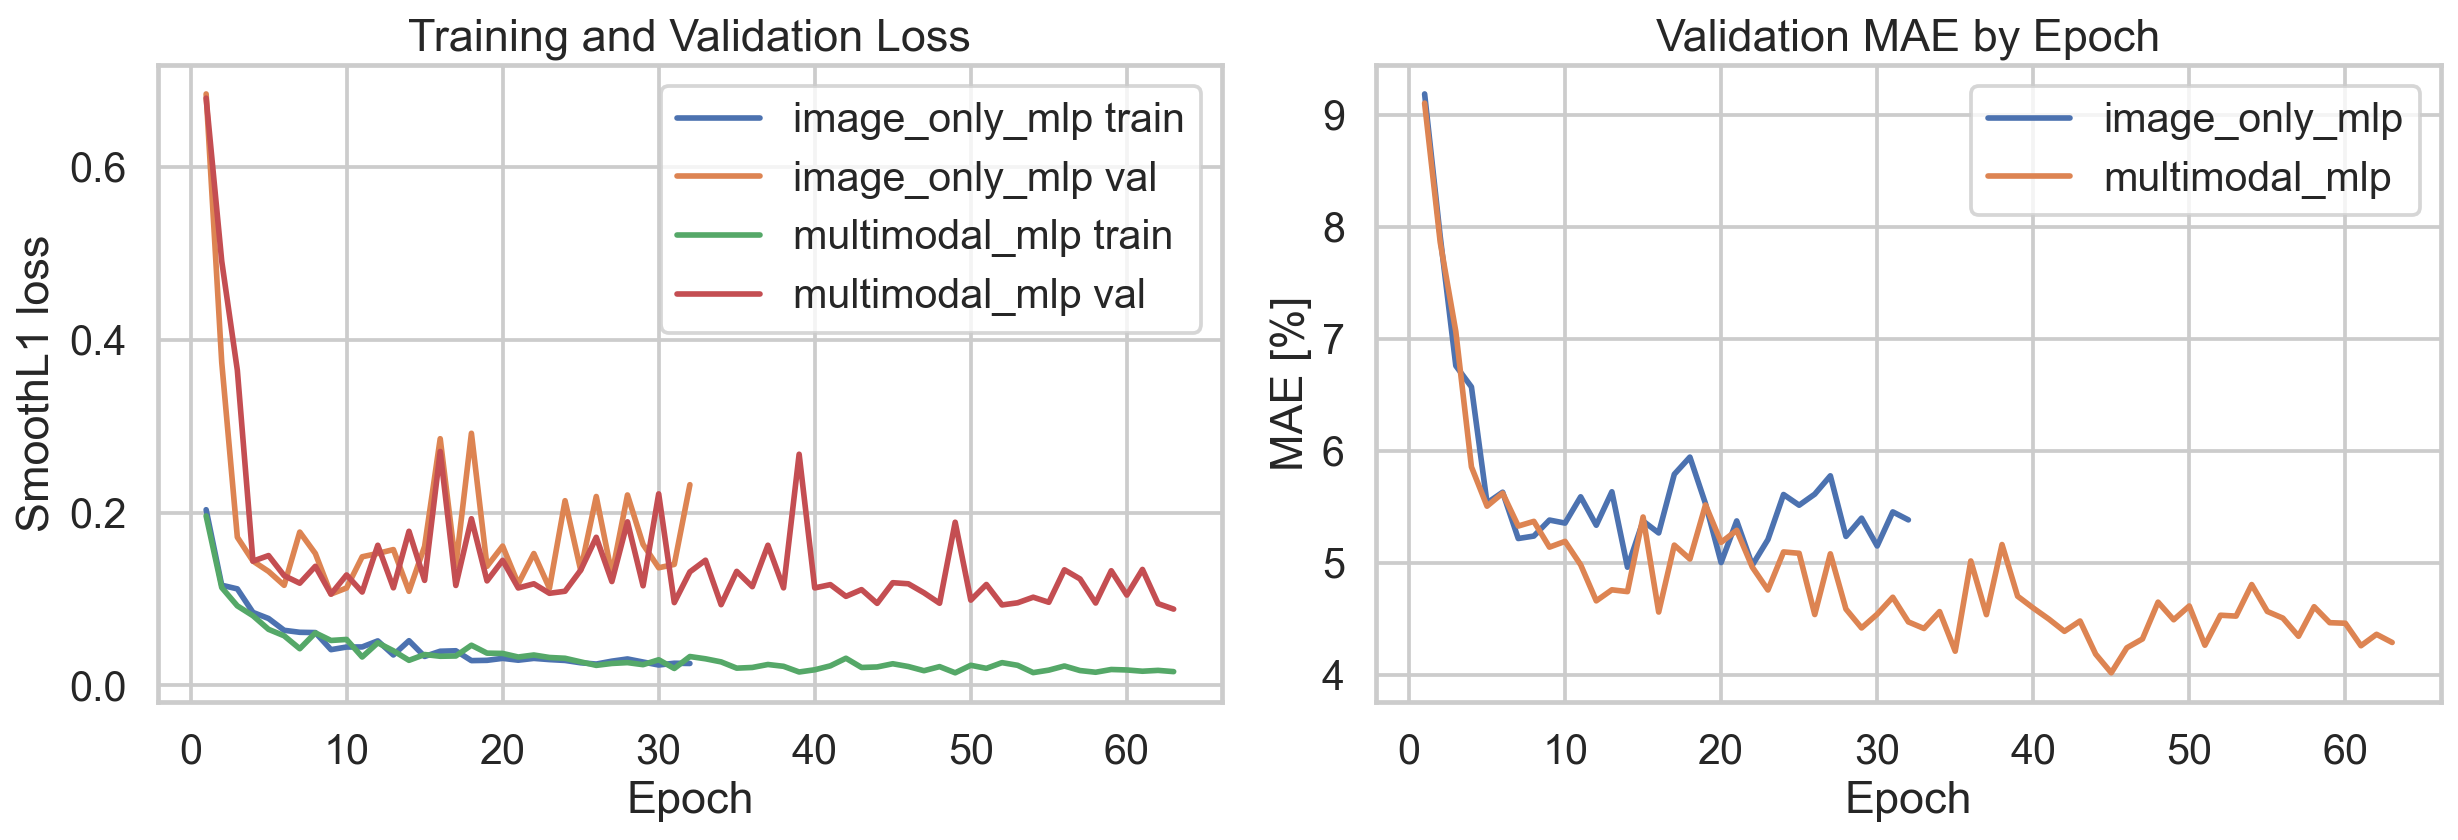
\includegraphics[width=0.92\textwidth]{reports/figures/00_learning_curves.png}
\caption{Training and validation curves for the two regression models. The multimodal branch reaches the lower validation MAE, but that did not translate into the better held-out test MAE.}
\label{fig:learning_curves}
\end{figure}

\begin{figure}[H]
\centering
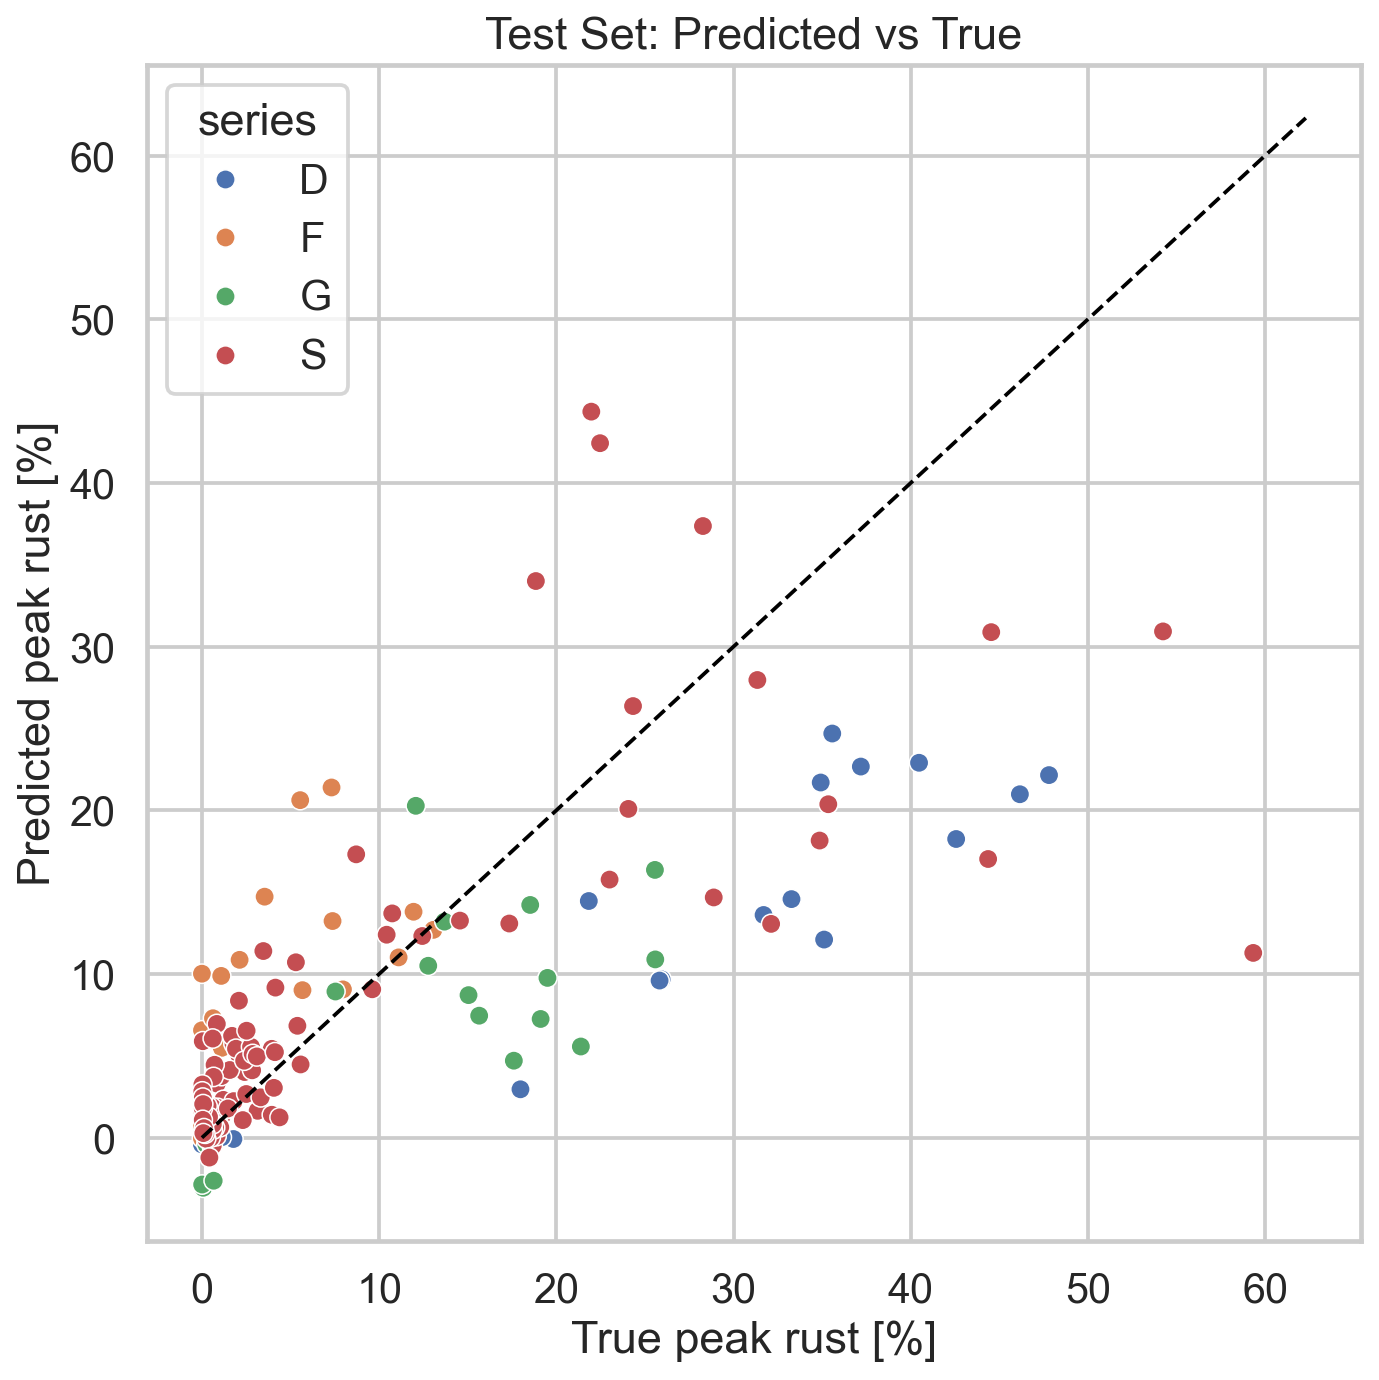
\includegraphics[width=0.72\textwidth]{reports/figures/02_pred_vs_true_test.png}
\caption{Predicted versus true peak rust on the grouped test split. The spread widens at higher rust values, and severe cases are often underpredicted.}
\label{fig:pred_vs_true}
\end{figure}

\begin{figure}[H]
\centering
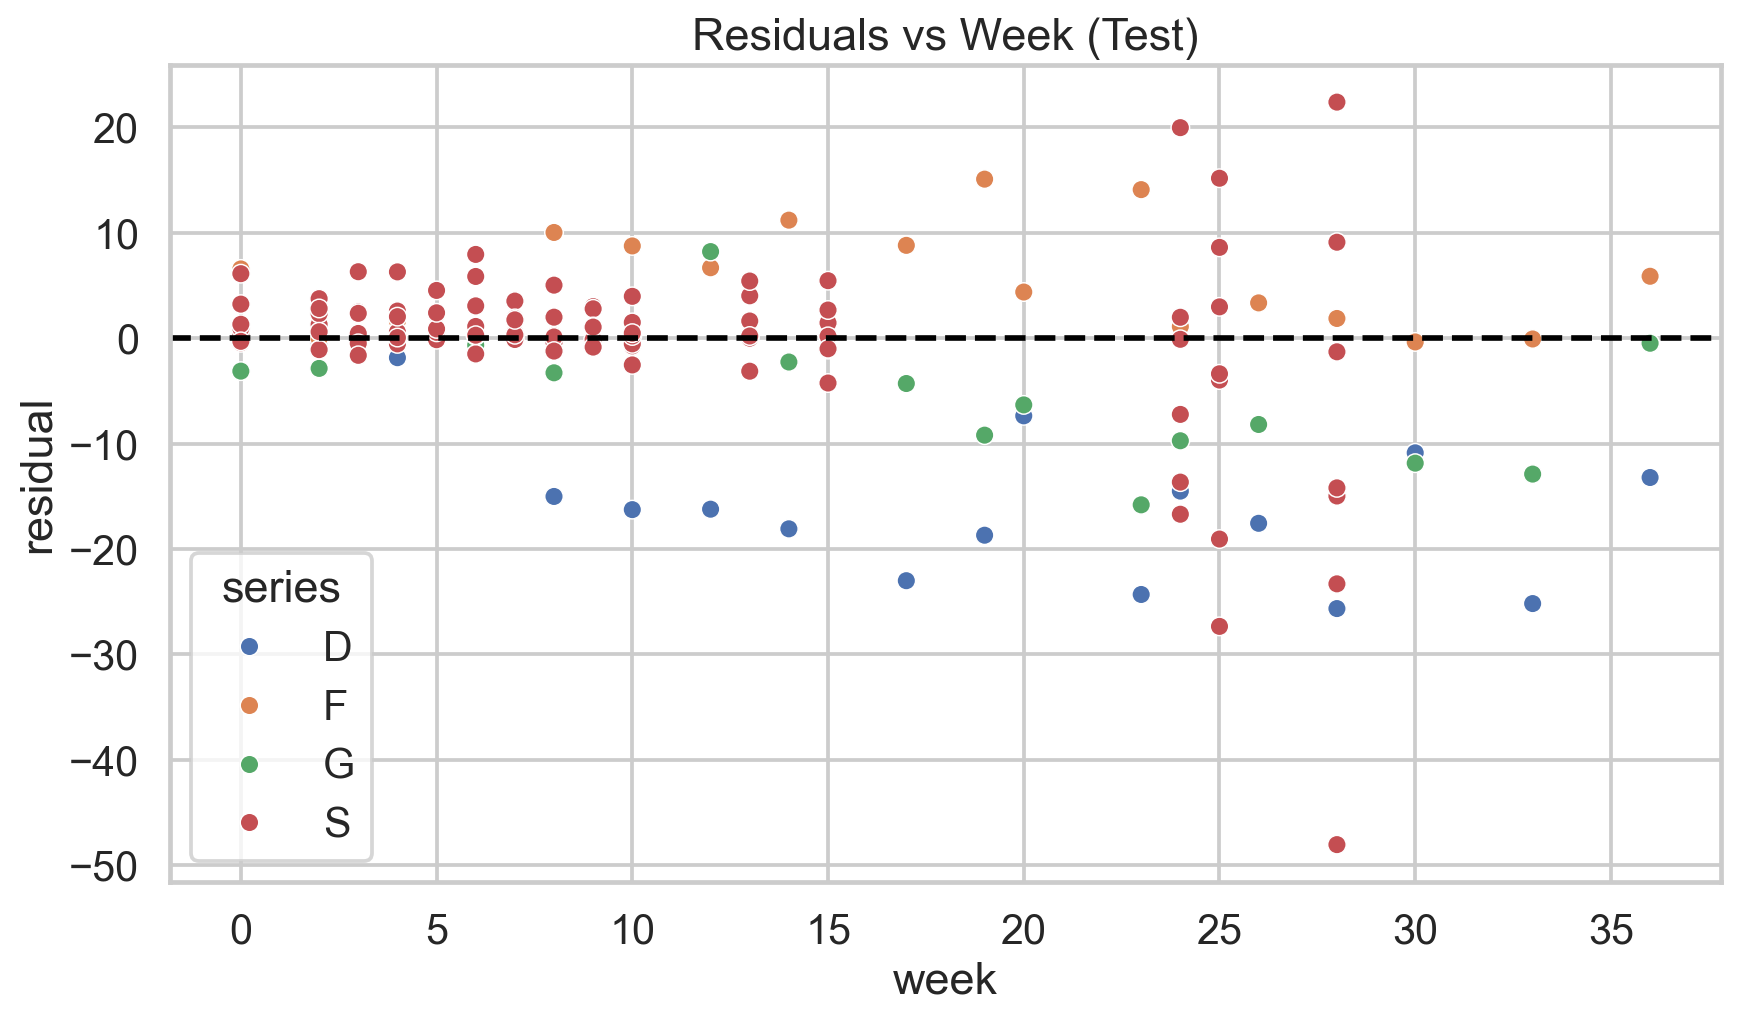
\includegraphics[width=0.84\textwidth]{reports/figures/04_residual_vs_week.png}
\caption{Residuals versus week on the grouped test split. Errors are small near week 0 and become increasingly negative at later weeks, indicating underprediction of severe late-stage corrosion.}
\label{fig:residual_vs_week}
\end{figure}

\begin{figure}[H]
\centering
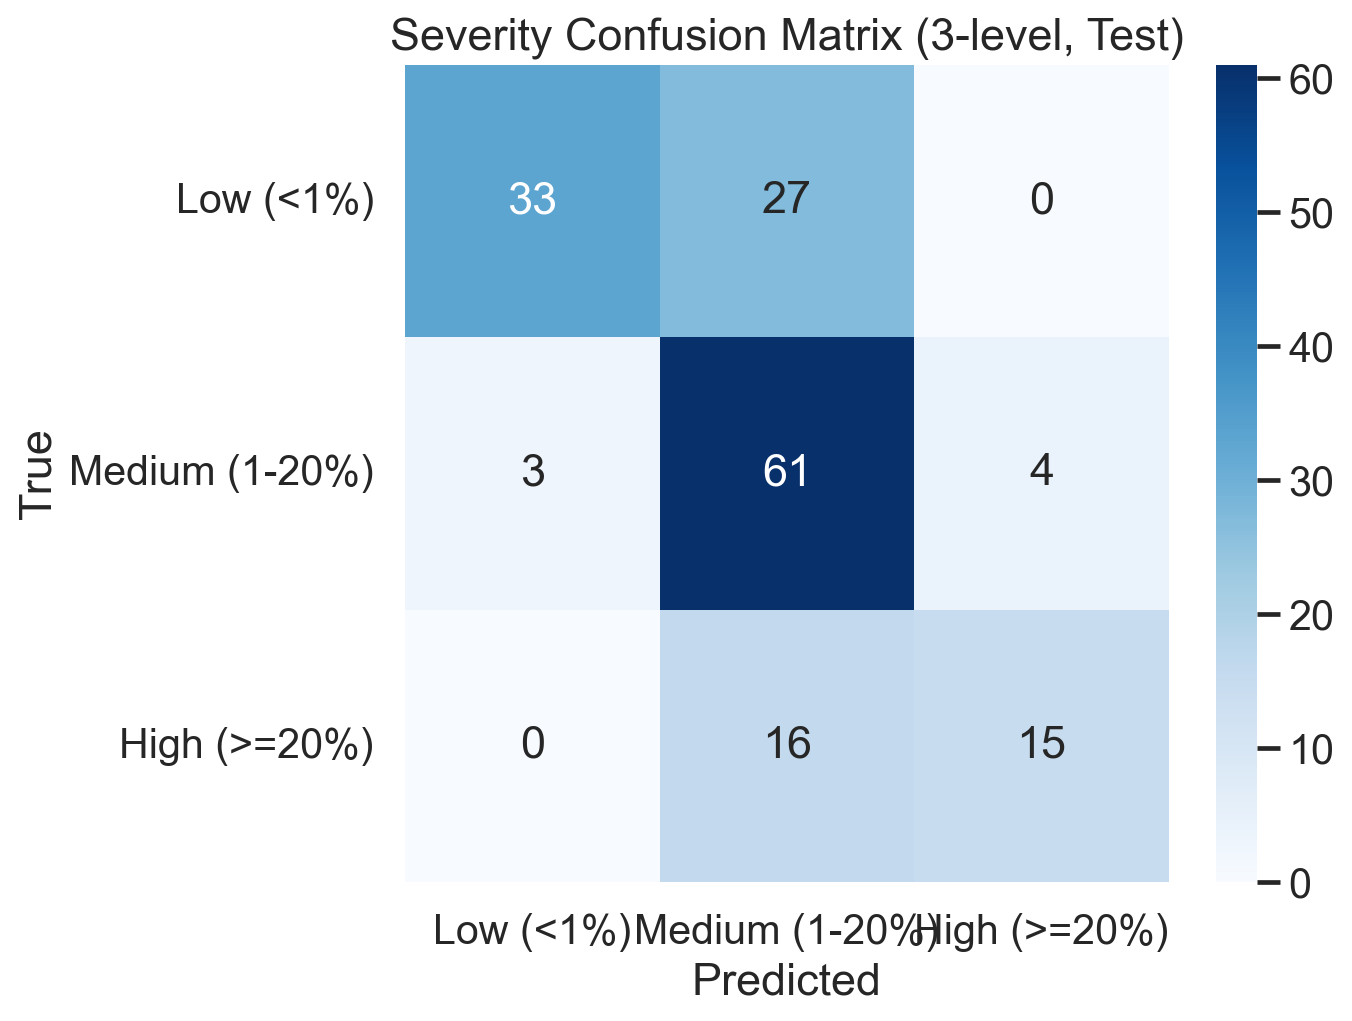
\includegraphics[width=0.66\textwidth]{reports/figures/10_severity_confusion_matrix.png}
\caption{Three-level severity confusion matrix generated from the regression output using thresholds \(<1\%\), \(1\%-<20\%\), and \(\geq20\%\). The model is strongest in the medium band and weaker at both extremes.}
\label{fig:severity_confusion}
\end{figure}

\begin{figure}[H]
\centering
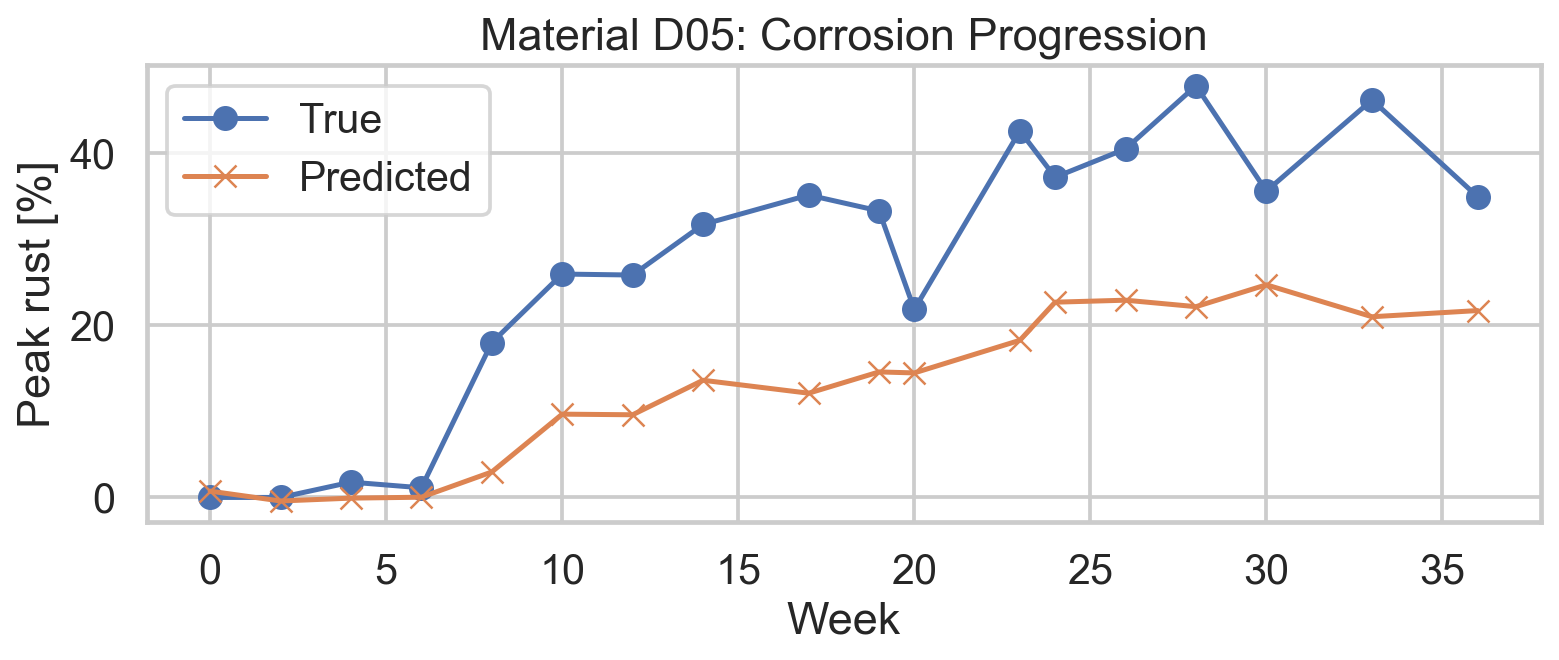
\includegraphics[width=0.88\textwidth]{reports/figures/per_material/D05_progression.png}
\caption{Per-specimen trajectory diagnostic for test specimen D05. This plot compares fitted values with already observed weekly labels; it is not a forecast trajectory. The model systematically underestimates the severe late-stage rise for this specimen.}
\label{fig:d05_progression}
\end{figure}

\subsection{Strongly supported results}
\paragraph{1. The selected model learns current visible corrosion reasonably well under grouped specimen holdout.}
The saved image-only model achieves test MAE 5.6255, test RMSE 9.2639, and \(R^2 = 0.5237\) on the grouped test split. This is the strongest technically supported performance statement in \texttt{main\_2}.

\paragraph{2. The dominant saved signal is image-driven, not multimodal.}
The final selected artifact uses only image embeddings (\texttt{use\_tabular = false}). Therefore the headline result in this repository is not that metadata fusion improved performance, but that the frozen visual representation alone slightly outperformed metadata fusion on the saved grouped test split.

\paragraph{3. Medium-severity corrosion is easier than the extremes.}
From the saved confusion matrix, overall three-level severity accuracy is 68.6\%. Class recall is 0.550 for low, 0.897 for medium, and 0.484 for high. The model is therefore best at coarse medium-range discrimination and weaker at both ends.

\subsection{Weak, negative, and inconclusive results}
\paragraph{Weak result: late-stage severe corrosion is underestimated.}
The saved test predictions show a clear late-week deterioration:
\begin{itemize}
  \item for weeks \(\leq 10\): MAE 2.220, bias \(+0.854\);
  \item for weeks 12--20: MAE 6.617, bias \(-1.314\);
  \item for weeks \(\geq 23\): MAE 12.075, bias \(-6.912\).
\end{itemize}
This pattern is visible in Figure~\ref{fig:residual_vs_week} and in the D05 specimen trajectory in Figure~\ref{fig:d05_progression}. The model becomes increasingly conservative as corrosion severity grows.

\paragraph{Weak result: performance is group-dependent.}
Group metrics computed on the test subset show substantial heterogeneity:
\begin{itemize}
  \item best treatment MAE: \texttt{SA\_VF}, 3.62;
  \item worst treatment MAE: \texttt{NO}, 8.18;
  \item best series MAE: S, 4.08;
  \item worst series MAE: D, 13.89;
  \item worst specimen MAE: D05, 13.89.
\end{itemize}
This means the single headline MAE hides materially different behavior across specimen families.

\paragraph{Negative result: the multimodal model did not win on the held-out grouped test split.}
Although the multimodal branch reached a better best validation MAE (4.0161 versus 4.9595), its test MAE was worse (5.7476 versus 5.6255). This prevents any supported claim that metadata fusion improved robustness in \texttt{main\_2}.

\paragraph{Negative result: offline predictions include physically impossible negatives.}
The saved prediction CSV contains 117 negative predictions in train, 7 in validation, and 13 in test, with a test minimum of \(-3.06\%\). Since the API path clips to \([0,100]\) but the offline CSV does not, the repository currently has inconsistent output semantics.

\paragraph{Inconclusive result: relationship to structural damage or residual capacity.}
No structural label is modeled in \texttt{main\_2}, so the corrosion-regression results cannot be promoted into claims about internal wire loss, ultimate load, or hidden degradation progression. The repository provides no output that directly tests those quantities here.

\subsection{What the results do \emph{not} justify claiming}
The saved outputs do not justify claiming that \texttt{main\_2}:
\begin{itemize}
  \item predicts RUL or failure time;
  \item predicts internal corrosion mechanisms from images;
  \item robustly generalizes across unseen campaigns or treatments;
  \item reproduces the thesis RGB-threshold workflow;
  \item demonstrates that multimodal fusion is superior;
  \item provides a clean, unbiased final test estimate, because test data were also used for model choice.
\end{itemize}

\section{What the model can and cannot learn}

\subsection{What is directly visible and therefore learnable}
From the images alone, the model can plausibly learn:
\begin{itemize}
  \item rust color and stain intensity;
  \item the spatial spread of visible corrosion evidence;
  \item coarse texture differences associated with clean versus corroded regions;
  \item specimen-level appearance patterns that correlate with treatment family or ageing stage.
\end{itemize}

Because the target itself is \texttt{B\_Peak\_Rust\_Percentage\_[\%]}, which is a same-surface visible corrosion label, this is a relatively favorable target for an image model. The task is narrower than predicting hidden internal damage.

\subsection{What may be indirectly inferable}
Through either image appearance or metadata, the pipeline may indirectly infer:
\begin{itemize}
  \item approximate exposure stage, since later weeks often exhibit greater visible corrosion;
  \item treatment family, either from the metadata branch or from systematic visual differences;
  \item campaign family, via \texttt{series} in the multimodal branch or via shared appearance characteristics.
\end{itemize}

However, such indirect inference is scientifically weaker than direct mechanistic estimation. It may reflect dataset structure rather than transferable physical understanding.

\subsection{What is hidden and likely not reliably recoverable here}
The current \texttt{main\_2} dataset and code do not support reliable recovery of:
\begin{itemize}
  \item internal wire loss at each week;
  \item ultimate load at each week;
  \item failure probability or time-to-threshold;
  \item causal degradation dynamics under new treatment schedules;
  \item robust extrapolation beyond the observed image-preprocessing regime.
\end{itemize}

These quantities are either hidden from the surface image, sparsely labeled only at specimen endpoints, or not represented at all in the executable training task.

\subsection{Why metadata can help but also mislead}
Metadata such as week, series, treatment, saline condition, and cover thickness can encode real mechanistic information. In a small dataset, they can also act as shortcuts by partially revealing expected corrosion level. The multimodal model's lower validation MAE but worse test MAE is consistent with this trade-off: metadata likely carries signal, but the repository does not show that it generalizes more robustly than image-only prediction.

\subsection{Scientific implication}
Scientifically, \texttt{main\_2} should be interpreted as a visible-corrosion quantification tool, not as a full structural health monitoring solution. It may be useful for automated scoring of current surface rust severity, but that is narrower than predicting hidden damage or remaining service life.

\section{Traceability to the original thesis and documentation}

\subsection{Documented method versus executable repository}
The local thesis PDF and conference paper describe a workflow centered on manual or semi-automated image preprocessing and rule-based corrosion extraction:
\begin{itemize}
  \item the thesis describes GIMP cropping, white-balance correction, BIMP batch preprocessing, and MATLAB RGB-threshold masking for automated corrosion analysis;
  \item the conference paper describes a MATLAB RGB-based classification workflow and a ResNet-50 classifier trained on corrosion classes derived from that process.
\end{itemize}

By contrast, \texttt{main\_2} implements a different computational path: frozen ResNet-18 embeddings, an MLP regressor, and a continuous peak-rust target.

\begin{table}[H]
\centering
\small
\begin{tabularx}{\textwidth}{p{0.28\textwidth} p{0.30\textwidth} Y}
\toprule
\textbf{Original documentation} & \textbf{What \texttt{main\_2} actually reproduces} & \textbf{Expected consequence of the mismatch} \\
\midrule
GIMP/BIMP preprocessing with cropping, white balance, and fixed export settings (thesis) & Not reproduced in executable code. \texttt{main\_2} relies on existing PNGs and torchvision transforms only. & Color-sensitive corrosion cues may shift if the current PNG set was not produced under the same preprocessing rules. \\
MATLAB RGB-threshold masking and binary segmentation (thesis/conference) & Not implemented in \texttt{main\_2}. No masks, no RGB thresholds, no strip counting. & Feature semantics differ substantially; \texttt{main\_2} cannot be claimed as a code reproduction of that pipeline. \\
Strip-based quantification along specimen length (conference) & Not implemented in \texttt{main\_2}. & Localized corrosion structure used in the documented method is absent from the executable feature set. \\
ResNet-50 image classification of corrosion classes (conference) & Not reproduced. \texttt{main\_2} uses frozen ResNet-18 embeddings plus regression. & Reported results are not directly comparable to conference classification metrics. \\
Image-based corrosion categorization into three levels (conference) & Only approximated post hoc by thresholding continuous regression outputs at 1\% and 20\%. & Severity confusion in \texttt{main\_2} is a diagnostic convenience, not the native supervised task. \\
792-image thesis dataset & Partially reproduced through saved artifacts, but the current raw workbook now exposes only 791 labeled rows; one corrupted image row remains only in the saved outputs and image directory. & Fresh reruns and exact traceability to the original data snapshot are currently broken. \\
\bottomrule
\end{tabularx}
\caption{Repository-grounded comparison between the documented project method and the executable \texttt{main\_2} code.}
\label{tab:traceability}
\end{table}

\subsection{What could not be recovered}
The repository does not contain the original GIMP/BIMP configuration files, the MATLAB code used for RGB-threshold corrosion masking, or a documented mapping from the current raw workbook to the \texttt{NaCl\%} feature expected by \texttt{main\_2}. Therefore the exact preprocessing and feature-generation steps described in the documentation cannot be fully reconstructed from the current repository state.

\subsection{How the report handles these mismatches}
Whenever documentation claims are broader than the code, this report defers to the code and saved artifacts. Where the code itself can no longer be rerun from the current raw workbook, the report states that ambiguity explicitly rather than inferring undocumented repair steps.

\section{Limitations}

The main limitations of \texttt{main\_2} are not generic; they are specific to the repository evidence:
\begin{enumerate}
  \item \textbf{Small specimen count.} The saved run uses 48 specimens, even though the row count is 792. Grouped generalization is therefore estimated from only 10 test specimens.
  \item \textbf{Imbalanced corrosion regime.} Stored category counts are dominated by low-rust observations, especially for the surface-rust category.
  \item \textbf{Late-stage underprediction.} Severe late-week corrosion is systematically underestimated, especially for D-series specimens.
  \item \textbf{No structural supervision in the executable task.} Structural endpoint labels exist but are sparse, specimen-terminal, and unused.
  \item \textbf{No direct RUL supervision.} Neither the data interface nor the code contains time-to-failure labels or threshold-crossing logic.
  \item \textbf{Current reproducibility drift.} The present workbook schema no longer matches the loader; the present API metadata points to another machine; the saved run therefore cannot be reproduced end to end without repair.
  \item \textbf{Potential metadata confounding.} The multimodal branch includes group identity and exposure-stage features that can encode shortcuts.
  \item \textbf{Test-set model selection.} The code uses the test split for model choice, so the final test metric is not a clean untouched estimate.
  \item \textbf{Output-range inconsistency.} Offline saved predictions are unclipped and can be negative, while API outputs are clipped to \([0,100]\).
  \item \textbf{Limited external validity.} Because image alignment and thesis-style preprocessing are not reproduced in code, transfer to differently prepared image sets is uncertain.
\end{enumerate}

\section{Future work}

The next steps that logically follow from the current \texttt{main\_2} evidence are technical repair and scope clarification, not generic model escalation:
\begin{enumerate}
  \item \textbf{Repair the data contract.} Update the loader to handle the current two-header workbook, parse row identifiers from \texttt{Sample Name}, and make the provenance of \texttt{NaCl\%} explicit.
  \item \textbf{Create an immutable manifest.} Freeze a CSV manifest that maps every PNG to its label row, including a documented decision for the corrupted image \texttt{E01-20240508-17W}.
  \item \textbf{Make artifact paths relative or relocatable.} Replace absolute path storage in \texttt{run\_info.json} so that inference and API deployment work on a different machine.
  \item \textbf{Separate model selection from test reporting.} Choose the final branch on validation only, then retrain or refit according to a documented protocol before final testing.
  \item \textbf{Constrain regression outputs.} Use bounded output heads or consistent clipping so that offline and deployed semantics agree.
  \item \textbf{Add stricter evaluation.} If robust transfer matters, add leave-one-series-out, leave-one-treatment-out, or campaign-forward splits instead of only grouped random splitting.
  \item \textbf{If the goal is thesis reproducibility, reintroduce the documented preprocessing.} Port or recover the GIMP/BIMP/MATLAB workflow, then compare the RGB-threshold features against the current deep-embedding approach.
  \item \textbf{If the goal is structural degradation or RUL, build a separate label strategy first.} Current \texttt{main\_2} does not contain the supervision needed for that objective.
\end{enumerate}

\appendix

\section{Meeting-defense questions and concise evidence-based answers}

\paragraph{Why not direct RUL?}
Because \texttt{main\_2} never defines an RUL target, never fits threshold-crossing time, and never trains a time-to-event model. The only supervised target is current \texttt{B\_Peak\_Rust\_Percentage\_[\%]}.

\paragraph{Why are grouped specimen splits necessary?}
Each specimen is imaged repeatedly across weeks. Random row-wise splitting would place closely related images of the same physical specimen into both train and test, which would inflate performance.

\paragraph{Why did the multimodal model not become the final artifact?}
The saved run shows lower validation MAE for the multimodal branch but lower \emph{test} MAE for the image-only branch. The code selects the model with lower test MAE, so the saved artifact is image-only.

\paragraph{Why does robustness appear to drop at higher corrosion levels?}
Late-stage test rows have much larger error and a strongly negative bias. High-severity recall in the three-level confusion matrix is only 0.484, and specimen D05 is a concrete example of severe underprediction.

\paragraph{Why can visible corrosion be predicted better than structural degradation?}
The target in \texttt{main\_2} is itself a visible surface label, so the image contains direct evidence for it. Structural variables are hidden, much sparser, and not supervised in the executable task.

\paragraph{How much of the signal comes from metadata?}
The repository does not provide a clean variance decomposition. What is observable is that metadata was strong enough to improve validation MAE in the multimodal branch, but not strong enough to beat image-only on the saved grouped test split.

\paragraph{What are the highest-risk assumptions in the current repository state?}
The largest risks are: the workbook-schema assumption in the loader, the use of stale absolute artifact paths, the use of the test set for model selection, and the implicit assumption that the current PNGs still reflect the documented thesis preprocessing.

\paragraph{Could preprocessing mismatch explain part of the failure?}
Yes. The documentation emphasizes cropping and white balance before corrosion analysis, but \texttt{main\_2} does not execute those steps. If the current PNG set differs from the documented preprocessing regime, the learned visual mapping can shift.

\paragraph{Which features are most interpretable?}
The tabular metadata are more interpretable than the 512-dimensional deep image embedding, but the selected saved artifact does not use them. The post-hoc low/medium/high severity bins are interpretable, but they are derived summaries rather than native model outputs.

\paragraph{What exactly do the reported metrics mean?}
MAE is the mean absolute error in percentage points of peak rust. RMSE penalizes larger errors more heavily. \(R^2\) measures variance explained on the saved grouped test split. The three-level confusion matrix is a secondary diagnostic produced by thresholding the regression output at 1\% and 20\%.

\paragraph{Can the API be used as-is today?}
Not without repair. The local artifacts exist, but \texttt{run\_info.json} points to absolute paths on another machine, so artifact loading fails in the current repository state.

\end{document}
